The Lake (LAK) Package computes the stage of each lake from a water balance: precipitation, evaporation, runoff, specified inflow and withdrawal, outlet flow, lake storage, and the lakebed seepage exchanged with the connected groundwater flow (GWF) cells \citep[\S 8]{modflow6gwf}. By default the package solves this balance for the stage with a substitution iteration nested inside each outer (Picard or Newton) iteration of the GWF solution: the stage is updated to balance its budget against the latest GWF heads, and the resulting seepage is then added to the GWF matrix. Because the stage lags the heads by one outer iteration, strongly coupled and steady-state lakes can require many outer iterations to converge, and some do not converge at all.

The \texttt{IMPLICIT} option instead adds each lake stage to the GWF matrix as an extra unknown (one row and column) and solves it together with the GWF heads. The lakebed seepage to each connected cell is assembled as a conductance coupling between the lake-stage row and the cell row. In the seepage, the lake stage and the connected-cell head are each kept greater than or equal to the lake bottom, the same wet/dry cutoff used by the default formulation, so the two formulations exchange the same seepage for a given stage and head. The remaining (non-seepage) budget terms are linearized in stage with a finite difference and added to the diagonal and right-hand side. Because the seepage is held at the lake bottom rather than smoothed, a Newton iteration can drive the stage of a drying lake below the lake bottom; activating Newton under-relaxation (the \texttt{UNDER\_RELAXATION} keyword on the model \texttt{NEWTON} option) relaxes such a stage back toward the bottom and is recommended for lakes that may dry, although it is not required for a lake that stays above its bottom. Because the stage is no longer lagged behind the heads, the implicit formulation is most advantageous when a strongly coupled lake begins far from equilibrium with the surrounding aquifer: the stronger the lakebed coupling, the more outer iterations the default formulation needs to work off the stage lag, whereas the implicit formulation solves the stage and the heads together and converges in far fewer -- a reduction that can exceed an order of magnitude. Lakes that the default formulation cannot bring to convergence are likewise routinely solved. The advantage narrows as a lake becomes weakly coupled or nearly disconnected and its stage is only loosely tied to the heads. The two examples below illustrate both regimes. At convergence the two formulations satisfy the same water balance and give equivalent heads, stages, and budgets.

\subsection{Perched (Disconnected) Lakes}

A lake is perched when the groundwater head at every connected cell falls below the lakebed, so all of its seepage is downward leakage. The lake-stage equation stays well posed only if its diagonal -- the derivative of the lake balance with respect to stage -- remains non-zero. Holding the connected-cell head at the lake bottom, once it has fallen below the lakebed, keeps this leakage dependent on the lake stage, because a deeper lake drives more leakage through its bed. The diagonal therefore stays non-zero as long as the lakebed retains appreciable leakance, and for a perched lake the implicit formulation determines a stage that matches the default formulation, which balances the same leakage. If the leakance itself becomes very small, however, the seepage conductance---and with it the lake-stage diagonal---becomes vanishingly small, and the implicit lake-stage equation can become too poorly conditioned for the coupled solver to advance on its own. To keep the implicit formulation robust in this limit, the package compares each lake's stage change with the change in its connected aquifer heads from one outer iteration to the next. A well-connected lake converges in step with its aquifer, so the two changes are comparable; a lake that has become the convergence bottleneck keeps changing its stage by much more than its connected heads, which have settled. When a lake's stage change persistently exceeds its connected head changes by a large factor, the package automatically switches that lake to the default substitution solver for the rest of that time step. The switch is reconsidered at the start of each time step, so a lake switched under one set of stresses can return to the implicit formulation in a later time step---for example, a transient period whose lake storage adds to the lake-stage diagonal and improves its conditioning. The substitution solver resolves the lake's one-dimensional water balance exactly within each outer iteration and is unconditionally robust, so the implicit formulation remains as reliable as the default formulation even as a lake approaches the disconnected state. A lake that genuinely benefits from the implicit coupling converges in step with its aquifer and is never switched. The decreasing-leakance example below illustrates this behavior.

One case still favors the default formulation: a lake whose connected cells dry and rewet under the standard rewetting (REWET) capability rather than the Newton formulation. Rewetting can settle on more than one valid configuration, so the implicit and default approaches, while both mass conserving, may reach different results. The Newton formulation keeps cells active and avoids this ambiguity, and is recommended for implicit lakes that may become perched.

\subsection{Examples}

The two formulations are compared with the Pleasant Lake local grid refinement (LGR) model (fig.~\ref{fig:pleasantdomain}), an example distributed with the Modflow-setup model-construction package \citep{leaf2022modflowsetup} that is derived from the Central Sands groundwater and lake-interaction study of \citet{fienen2022centralsands}. The model couples a 200~m parent grid to a 20~m inset grid, centered on Pleasant Lake, through a ghost-node-corrected GWF-GWF exchange; streamflow routing and a water mover connect the two models, and both use the Newton-Raphson formulation. The lake is represented in the inset model with 1{,}382 vertical lakebed connections. For these examples the original transient simulation was reduced to a single steady-state stress period, the lake stage was initialized about 8~m below its converged value, and both formulations were run from that same out-of-equilibrium stage with an outer dependent-variable closure criterion of $10^{-4}$~m and a maximum of 1{,}000 outer iterations.

The two examples vary the lakebed leakance of every lake connection from its calibrated value of $2.2 \times 10^{-3}$~d$^{-1}$ in opposite directions. The first increases the leakance to strengthen the coupling between the lake and the aquifer, the regime in which the default formulation's lagged stage is most costly and the implicit formulation reduces the iteration count the most. The second decreases the leakance to drive the lake toward a disconnected state, the regime in which the lake stage becomes weakly tied to the heads and the implicit formulation relies on its substitution fallback to remain robust.

\begin{figure}[!ht]
	\centering
	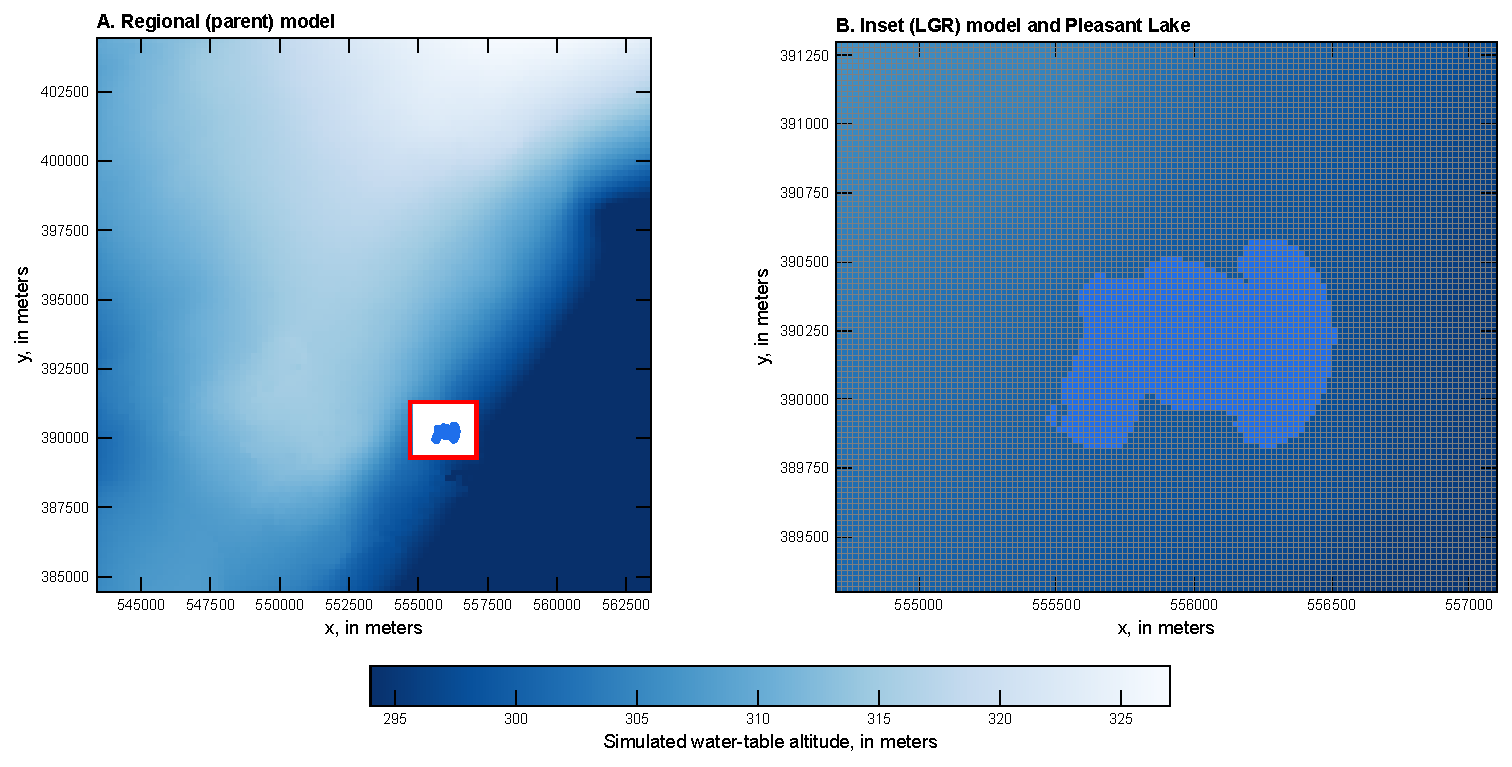
\includegraphics[width=\textwidth]{./Figures/PleasantLakeDomain.pdf}
	\caption[Pleasant Lake local grid refinement model domain]{Pleasant Lake local grid refinement (LGR) model: (\textit{A}) the regional parent model and simulated water-table altitude, with the inset (LGR) domain outlined in red; and (\textit{B}) the refined inset model and the simulated lake (blue cells). The model is an example distributed with the Modflow-setup package \citep{leaf2022modflowsetup} and is based on the Central Sands study of \citet{fienen2022centralsands}}
	\label{fig:pleasantdomain}
\end{figure}

\subsubsection{Strongly Coupled Lake}

The lakebed leakance of every lake connection was increased from its calibrated value by successive factors of ten, strengthening the coupling between the lake and the aquifer. Because the stage was started out of equilibrium, the default formulation must work the lagged stage back into balance with the heads, and the number of outer iterations it requires grows rapidly as the coupling strengthens (table~\ref{tab:lakestrong}). The implicit formulation solves the stage together with the heads and is nearly unaffected: at a leakance of $2.2 \times 10^{0}$~d$^{-1}$ the default formulation requires 585 outer iterations and the implicit formulation only 47, a reduction of more than an order of magnitude, and the run time falls correspondingly from 119 to 13~seconds. Both formulations converge to the same lake stage. The maximum head difference $\Delta h$ in the table grows with the coupling because the same outer closure criterion ($10^{-4}$~m) admits a larger absolute spread in a more strongly coupled (stiffer) system; tightening the criterion to $10^{-6}$~m reduces $\Delta h$ at the strongest coupling from $7.2 \times 10^{-3}$ to $1.3 \times 10^{-3}$~m, confirming that the two formulations converge to the same solution.

\begin{table}[!ht]
	\caption[Comparison of the default and implicit lake formulations as lakebed leakance is increased]{Number of outer iterations, converged lake stage, run time, and the maximum absolute difference $\Delta h$ in simulated inset-model heads between the default and implicit formulations of the Pleasant Lake example, as the lakebed leakance of every lake connection is increased from its calibrated value of $2.2 \times 10^{-3}$~d$^{-1}$ to strengthen the lake-aquifer coupling. As the coupling strengthens the default formulation requires rapidly increasing numbers of outer iterations to work off the lagged lake stage, whereas the implicit formulation is nearly unaffected; both formulations converge to the same lake stage}
	\label{tab:lakestrong}
	\small
	\centering
	\begin{tabular}{r rrr rrr r}
		\hline
		\hline
		& \multicolumn{3}{c}{Default} & \multicolumn{3}{c}{Implicit} & \\
		\cline{2-4} \cline{5-7}
		Leakance & Outer & Stage & Time & Outer & Stage & Time & $\Delta h$ \\
		(d$^{-1}$) & iter. & (m) & (s) & iter. & (m) & (s) & (m) \\
		\hline
		$2.2 \times 10^{-3}$ & 54 & 299.07 & 12.9 & 50 & 299.07 & 10.9 & $2.2 \times 10^{-4}$ \\
		$2.2 \times 10^{-2}$ & 123 & 298.86 & 25.5 & 106 & 298.86 & 17.8 & $8.7 \times 10^{-4}$ \\
		$2.2 \times 10^{-1}$ & 314 & 298.80 & 64.5 & 56 & 298.80 & 13.1 & $3.9 \times 10^{-3}$ \\
		$2.2 \times 10^{0}$ & 585 & 298.79 & 119.3 & 47 & 298.78 & 12.9 & $7.2 \times 10^{-3}$ \\
		\hline
		\hline
	\end{tabular}
\end{table}

\subsubsection{Decreasing Lakebed Leakance}

The lakebed leakance of every lake connection was reduced from its calibrated value by successive factors of ten to drive the lake progressively toward a disconnected state. Because the lake has a net positive inflow (precipitation exceeds evaporation) and no outlet, it can reach a steady state only by leaking the excess water to the aquifer through its bed; as the leakance is reduced, a larger head difference is required to pass that inflow, so the steady-state stage rises (table~\ref{tab:lakedisconnect}).

\begin{table}[!ht]
	\caption[Comparison of the default and implicit lake formulations as lakebed leakance is reduced]{Number of outer iterations, converged lake stage, run time, and the maximum absolute difference $\Delta h$ in simulated inset-model heads between the default and implicit formulations of the Pleasant Lake example, as the lakebed leakance of every lake connection is reduced from its calibrated value of $2.2 \times 10^{-3}$~d$^{-1}$. Both formulations converge at every leakance and agree on the lake stage and simulated heads; at the smaller leakances the implicit formulation converges by automatically switching the lake to the substitution solver}
	\label{tab:lakedisconnect}
	\small
	\centering
	\begin{tabular}{r rrr rrrc r}
		\hline
		\hline
		& \multicolumn{3}{c}{Default} & \multicolumn{4}{c}{Implicit} & \\
		\cline{2-4} \cline{5-8}
		Leakance & Outer & Stage & Time & Outer & Stage & Time & & $\Delta h$ \\
		(d$^{-1}$) & iter. & (m) & (s) & iter. & (m) & (s) & Conv. & (m) \\
		\hline
		$2.2 \times 10^{-3}$ & 54 & 299.07 & 12.9 & 50 & 299.07 & 10.9 & yes & $2.2 \times 10^{-4}$ \\
		$2.2 \times 10^{-4}$ & 51 & 300.41 & 11.3 & 60 & 300.41 & 11.6 & yes & $4.3 \times 10^{-5}$ \\
		$2.2 \times 10^{-5}$ & 51 & 313.22 & 11.2 & 52 & 313.22 & 11.9 & yes & $7.5 \times 10^{-6}$ \\
		$2.2 \times 10^{-6}$ & 51 & 441.28 & 10.9 & 44 & 441.28 & 10.7 & yes & $1.6 \times 10^{-5}$ \\
		$2.2 \times 10^{-7}$ & 51 & 1{,}721.8 & 11.3 & 43 & 1{,}721.8 & 11.0 & yes & $1.6 \times 10^{-5}$ \\
		$2.2 \times 10^{-8}$ & 51 & 14{,}527 & 11.1 & 280 & 14{,}527 & 82.5 & yes & $1.1 \times 10^{-4}$ \\
		$2.2 \times 10^{-9}$ & 51 & 142{,}584 & 11.2 & 286 & 142{,}584 & 82.7 & yes & $4.6 \times 10^{-5}$ \\
		\hline
		\hline
	\end{tabular}
\end{table}

Across the full range of leakances the two formulations converge to the same lake stage and agree on the simulated heads to better than $10^{-3}$~m (table~\ref{tab:lakedisconnect}). While the lake remains appreciably connected (the larger leakances), the implicit formulation solves the lake stage directly in the matrix and converges in a comparable number of outer iterations as the default formulation, or fewer. As the leakance is reduced and the lake-stage diagonal of the implicit system---supplied almost entirely by the lakebed seepage conductance for this lake---becomes vanishingly small, the stage can no longer be advanced as a matrix unknown: it keeps changing while its connected aquifer heads settle. The implicit formulation detects this imbalance and switches the lake to the substitution solver. For moderately disconnected lakes the switch occurs early and convergence stays comparable to the default formulation. For the most extreme disconnection, the lake stays in step with its slowly settling aquifer for many iterations before the imbalance becomes apparent, so the switch occurs later and the substitution solver needs several times as many outer iterations to bring the coupled system to balance; the implicit formulation still converges, but at a higher cost in this limit. The default formulation, which solves the one-dimensional lake water balance directly within each outer iteration, converges in about 50 outer iterations regardless of the leakance.

Both formulations are robust in this limit, but the converged stage is not physically meaningful. A lake that is hydraulically disconnected from the aquifer and has a net positive inflow with no outlet has no finite steady state; the stage that balances the vanishing seepage grows without bound as the leakance is reduced, reaching about $1.4 \times 10^{5}$~m at the smallest leakance tested. The robustness of the implicit formulation in this limit, provided by the substitution fallback, is a numerical convenience and not a physical result: a steady-state lake that is expected to become disconnected from the aquifer should be given an outlet or a transient representation so that the simulated stage remains physically meaningful.
